 
% Para una visualizacion correcta, generar el PDF
% Ni el DVI ni el PS se visualizan bien

% Elegir el estilo que se desee, hay cientos en la red

\documentclass{beamer}
\usepackage[spanish]{babel}
\usepackage[utf8]{inputenc}
\usepackage{tikz}
\usepackage{ragged2e} %Alineación de texto
\usepackage{etoolbox}
\usepackage{todonotes}
\usepackage{animate}

%\usetheme{Warsaw}
% \usetheme{Rochester}
%\usetheme{bars}
% \usetheme{Bergen}
% \usetheme{Boadilla}
% \usetheme{classic}
% \usetheme{Madrid}
% \usetheme{Pittsburgh}
% \usetheme{Antibes}
% \usetheme{Montpellier}
% \usetheme{Berkeley}
%\usetheme{PaloAlto}
% \usetheme{Goettingen}
% \usetheme{Marburg}
% \usetheme{Hannover}
%\usetheme{JuanLesPins}
% \usetheme{Berlin}
% \usetheme{Ilmenau}
\usetheme{shadow}
% \usetheme{Luebeck}
%\usetheme{Darmstadt}
% \usetheme{Frankfurt}
% \usetheme{Singapore}
%\usetheme{Szeged}
%\usetheme{Copenhagen}
% \usetheme{lined}
% \usetheme{Malmoe}
% \usetheme{shadow}
% \usetheme{sidebar}
% \usetheme{split}
% \usetheme{default}
%\usetheme{Dresden}
\usecolortheme{lily}
\usefonttheme{structurebold}

\setbeamerfont{title}{size=\huge,series=\bfseries,parent=structure}
\setbeamerfont{author}{size=\large,series=\bfseries,parent=structure}
%\setbeamerfont{institute}{size=\tiny}
%\beamertemplategridbackground[0.5cm]

\setbeamertemplate{navigation symbols}{}

\useoutertheme[footline,subsection=false]{miniframes}
\useinnertheme{circles}

\hypersetup{pdfpagemode=FullScreen}
\setbeamercovered{transparent}
\apptocmd{\frame}{}{\justifying}{}
\addtobeamertemplate{block begin}{}{\justifying}

\begin{document}
\titlegraphic{
\includegraphics[width=25mm]{images/logo_usc.eps}}
\title{Visualización de observacións en SIX de escritorio}
\author{Rubén Mosquera Varela}
\institute{Traballo de Fin de Grao en Enxeñaría Informática\\
\bigskip Directores: José Ramón Ríos Viqueira e Manuel Antonio Regueiro Seoane}
\date{Xullo de 2015}

%\addtobeamertemplate{frametitle}{}{
%\begin{tikzpicture}[remember picture,overlay]
%\node at([shift={(-0.6cm,-0.6cm)}]current page.north east) {
\includegraphics[height=.6cm,width=.6cm]{images/presentacion/sosclient.png}};
%\end{tikzpicture}}

\begin{frame}[plain]
	\transdissolve
	\titlepage
\end{frame}

\begin{frame}{Índice}
	\transdissolve
	\tableofcontents
\end{frame}

\section{Introdución}
\begin{frame}{Contextualización}{Sistema de información xeográfica}
	\onslide<1->{\begin{block}{Que é un SIX?}
	\begin{itemize}
	\item Sistema deseñado para capturar, almacenar, manipular, analizar e presentar calquera tipo de información xeograficamente referenciada.
	\item Usos: meteoroloxía, cartografía, hidroloxía, xestión de recursos, loxística, avaliación do impacto ambiental, etc.
	\end{itemize}
	\end{block}}
	\onslide<2->{\begin{block}{}
	\begin{columns}[T]
	\begin{column}{.3\textwidth}
	{\usebeamerfont{structure}{\usebeamercolor[fg]{structure} Exemplos}}
	\begin{itemize}
		\item<2->Geomedia
		\item<3->ArcGIS
		\item<4->gvSIG
		\item<5->QGIS
	\end{itemize}
	\end{column}
	\begin{column}{5cm}
	\begin{overprint}
		\only<1>{\begin{minipage}{3.5cm}\hfill\vspace{3.5cm} \end{minipage}}
		\includegraphics<2>[height=3.5cm]{images/presentacion/geomedia.jpg}
		\includegraphics<3>[height=3.5cm]{images/presentacion/ArcGIS.png}
		\includegraphics<4>[height=3.5cm]{images/presentacion/GvSIG.jpg}
		\includegraphics<5>[height=3.5cm]{images/presentacion/QGIS.png}
	\end{overprint}
	\end{column}
	\end{columns}
	\end{block}}
\end{frame}

\begin{frame}{Contextualización}{Observación medioambiental}
\onslide<1->
	{\begin{block}{Observación}
	\begin{columns}
	\begin{column}{.55\textwidth}\justifying
	É un evento que estima unha propiedade, nun momento concreto, dunha entidade de interese,
utilizando un procedemento especificado e que xera un resultado.
	\end{column}
	\begin{column}{.35\textwidth}
	\includegraphics<1->[width=\textwidth]{images/presentacion/OaM_4_dummies_2.png}
	\end{column}
	\end{columns}
	\end{block}}
\onslide<2->	
	{\begin{block}{}
	\begin{columns}[T]
	\begin{column}{.35\textwidth}\justifying
	{\usebeamerfont{structure}{\usebeamercolor[fg]{structure} Información ambiental}}
	\begin{itemize}
		\item<2-> Inxente e crecente volume
		\item<3-> Moi heteroxéneo
		\item<4-> Diversas axencias implicadas
	\end{itemize}
	\end{column}
	\begin{column}{.55\textwidth}
	\begin{overprint}
		\only<1>{\begin{minipage}{3cm}\hfill\vspace{3cm} \end{minipage}}
		\includegraphics<2>[height=3cm]{images/presentacion/estacionstemperatura.png}
		\includegraphics<3>[height=3cm]{images/presentacion/sensores.png}
		\includegraphics<4>[height=3cm]{images/presentacion/inspire.jpg}
	\end{overprint}
	\end{column}
	\end{columns}
	\end{block}}
\end{frame}

\begin{frame}{Contextualización}{Open Geospatial Consortium (OGC)}
\onslide<1->{
\begin{block}{Open Geospatial Consortium (OGC)}
Consorcio internacional co obxectivo de desenvolver e publicar estándares no eido da información xeoespacial
\end{block}}
\onslide<2->{
\begin{block}{Sensor Web Enablement (SWE)}
		\onslide<3->{
		Sensor Observation Service (SOS)
		\begin{itemize}
		\item GetCapabilities
		\item DescribeSensor
		\item GetObservations
		\end{itemize}}
		\onslide<4->{
		Observations\&Measurements (O\&M)
		\begin{itemize}
		\item Observations
		\item Measurements
		\end{itemize}}
\end{block}}
\end{frame}

\begin{frame}{Motivación}{}
	{\begin{block}{Motivación}
	Inexistencia dun sistema de información xeográfica libre e de propósito xeral que permita a incorporación e análise de datos de observacións dispoñibles a través da interface SOS.\end{block}}
\end{frame}

\begin{frame}{Obxectivos}{}
	{\begin{block}{Obxectivos}
	Desenvolvemento dunha extensión para a ferramenta SIX libre QGIS que permita a conexión a fontes de datos SOS e a exploración dos seus contidos no contorno de mapas proporcionado pola ferramenta.
	\begin{itemize}
	\item<2->Interacción co SOS para a obtención dos datos de sensores e as observacións realizadas polos mesmos.
	\item<3->Procesamento dos datos obtidos a través dos servizos SOS para a súa adecuación á estrutura de datos manexada por QGIS.
	\item<4->Dotar á ferramenta das utilidades necesarias para interaccionar comodamente con datos en series temporais ou variables multidimensionais.
	\end{itemize}
	\end{block}}
\end{frame}

\section{Deseño do software}
\begin{frame}{Arquitectura do sistema}{Visión estática}
\begin{block}{}
\begin{overprint}
	\only<1>{\centerline{\includegraphics[width=0.50\linewidth]{images/presentacion/componentes0.eps}}}
	\only<2>{\centerline{\includegraphics[width=0.50\linewidth]{images/presentacion/componentes1.eps}}}
	\only<3>{\centerline{\includegraphics[width=0.50\linewidth]{images/presentacion/componentes2.eps}}}
\end{overprint}
\end{block}
\end{frame}

\begin{frame}{Arquitectura do sistema}{Visión dinámica}
\begin{block}
\centering
\ifx\du\undefined
  \newlength{\du}
\fi
\setlength{\du}{6.5\unitlength}
\begin{tikzpicture}
\pgftransformxscale{1.000000}
\pgftransformyscale{-1.000000}
\definecolor{dialinecolor}{rgb}{0.000000, 0.000000, 0.000000}
\pgfsetstrokecolor{dialinecolor}
\definecolor{dialinecolor}{rgb}{1.000000, 1.000000, 1.000000}
\pgfsetfillcolor{dialinecolor}
\pgfsetlinewidth{0.100000\du}
\pgfsetdash{}{0pt}
\definecolor{dialinecolor}{rgb}{1.000000, 1.000000, 1.000000}
\pgfsetfillcolor{dialinecolor}
\pgfpathellipse{\pgfpoint{7.145000\du}{3.945000\du}}{\pgfpoint{0.300000\du}{0\du}}{\pgfpoint{0\du}{0.300000\du}}
\pgfusepath{fill}
\definecolor{dialinecolor}{rgb}{0.000000, 0.000000, 0.000000}
\pgfsetstrokecolor{dialinecolor}
\pgfpathellipse{\pgfpoint{7.145000\du}{3.945000\du}}{\pgfpoint{0.300000\du}{0\du}}{\pgfpoint{0\du}{0.300000\du}}
\pgfusepath{stroke}
\definecolor{dialinecolor}{rgb}{0.000000, 0.000000, 0.000000}
\pgfsetstrokecolor{dialinecolor}
\draw (5.945000\du,4.545000\du)--(8.345000\du,4.545000\du);
\definecolor{dialinecolor}{rgb}{0.000000, 0.000000, 0.000000}
\pgfsetstrokecolor{dialinecolor}
\draw (7.145000\du,4.245000\du)--(7.145000\du,5.745000\du);
\definecolor{dialinecolor}{rgb}{0.000000, 0.000000, 0.000000}
\pgfsetstrokecolor{dialinecolor}
\draw (7.145000\du,5.745000\du)--(5.945000\du,7.045000\du);
\definecolor{dialinecolor}{rgb}{0.000000, 0.000000, 0.000000}
\pgfsetstrokecolor{dialinecolor}
\draw (7.145000\du,5.745000\du)--(8.345000\du,7.045000\du);
% setfont left to latex
\definecolor{dialinecolor}{rgb}{0.000000, 0.000000, 0.000000}
\pgfsetstrokecolor{dialinecolor}
\node at (7.145000\du,8.240000\du){{\tiny Usuario}};
\pgfsetlinewidth{0.100000\du}
\pgfsetdash{}{0pt}
\definecolor{dialinecolor}{rgb}{1.000000, 1.000000, 1.000000}
\pgfsetfillcolor{dialinecolor}
\fill (17.654500\du,6.645000\du)--(17.654500\du,8.445000\du)--(20.252000\du,8.445000\du)--(20.252000\du,6.645000\du)--cycle;
\definecolor{dialinecolor}{rgb}{0.000000, 0.000000, 0.000000}
\pgfsetstrokecolor{dialinecolor}
\draw (17.654500\du,6.645000\du)--(17.654500\du,8.445000\du)--(20.252000\du,8.445000\du)--(20.252000\du,6.645000\du)--cycle;
% setfont left to latex
\definecolor{dialinecolor}{rgb}{0.000000, 0.000000, 0.000000}
\pgfsetstrokecolor{dialinecolor}
\node at (18.953250\du,7.740000\du){{\tiny QGIS}};
% setfont left to latex
\pgfsetlinewidth{0.050000\du}
\definecolor{dialinecolor}{rgb}{0.000000, 0.000000, 0.000000}
\pgfsetstrokecolor{dialinecolor}
%\draw (18.154500\du,7.892500\du)--(19.752000\du,7.892500\du);
\pgfsetlinewidth{0.100000\du}
\pgfsetdash{}{0pt}
\definecolor{dialinecolor}{rgb}{1.000000, 1.000000, 1.000000}
\pgfsetfillcolor{dialinecolor}
\fill (28.629800\du,6.595000\du)--(28.629800\du,8.395000\du)--(34.842300\du,8.395000\du)--(34.842300\du,6.595000\du)--cycle;
\definecolor{dialinecolor}{rgb}{0.000000, 0.000000, 0.000000}
\pgfsetstrokecolor{dialinecolor}
\draw (28.629800\du,6.595000\du)--(28.629800\du,8.395000\du)--(34.842300\du,8.395000\du)--(34.842300\du,6.595000\du)--cycle;
% setfont left to latex
\definecolor{dialinecolor}{rgb}{0.000000, 0.000000, 0.000000}
\pgfsetstrokecolor{dialinecolor}
\node at (31.736050\du,7.690000\du){{\tiny SOSClientDlg}};
% setfont left to latex
\pgfsetlinewidth{0.050000\du}
\definecolor{dialinecolor}{rgb}{0.000000, 0.000000, 0.000000}
\pgfsetstrokecolor{dialinecolor}
%\draw (29.129800\du,7.842500\du)--(34.342300\du,7.842500\du);
\pgfsetlinewidth{0.050000\du}
\pgfsetdash{}{0pt}
\pgfsetdash{{0.400000\du}{0.400000\du}}{0\du}
\definecolor{dialinecolor}{rgb}{0.000000, 0.000000, 0.000000}
\pgfsetstrokecolor{dialinecolor}
\draw (7.145000\du,8.445000\du)--(7.145000\du,9.545000\du);
\definecolor{dialinecolor}{rgb}{0.000000, 0.000000, 0.000000}
\pgfsetstrokecolor{dialinecolor}
\draw (7.145000\du,32.045000\du)--(7.145000\du,33.245000\du);
\pgfsetlinewidth{0.100000\du}
\pgfsetdash{}{0pt}
\definecolor{dialinecolor}{rgb}{1.000000, 1.000000, 1.000000}
\pgfsetfillcolor{dialinecolor}
\fill (6.795000\du,9.545000\du)--(6.795000\du,32.045000\du)--(7.495000\du,32.045000\du)--(7.495000\du,9.545000\du)--cycle;
\definecolor{dialinecolor}{rgb}{0.000000, 0.000000, 0.000000}
\pgfsetstrokecolor{dialinecolor}
\draw (6.795000\du,9.545000\du)--(6.795000\du,32.045000\du)--(7.495000\du,32.045000\du)--(7.495000\du,9.545000\du)--cycle;
\pgfsetlinewidth{0.120000\du}
\definecolor{dialinecolor}{rgb}{0.000000, 0.000000, 0.000000}
\pgfsetstrokecolor{dialinecolor}
\draw (7.945000\du,34.045000\du)--(6.345000\du,32.445000\du);
\definecolor{dialinecolor}{rgb}{0.000000, 0.000000, 0.000000}
\pgfsetstrokecolor{dialinecolor}
\draw (7.945000\du,32.445000\du)--(6.345000\du,34.045000\du);
\pgfsetlinewidth{0.050000\du}
\pgfsetdash{}{0pt}
\pgfsetdash{{0.400000\du}{0.400000\du}}{0\du}
\definecolor{dialinecolor}{rgb}{0.000000, 0.000000, 0.000000}
\pgfsetstrokecolor{dialinecolor}
\draw (18.953200\du,8.445000\du)--(18.953200\du,9.545000\du);
\definecolor{dialinecolor}{rgb}{0.000000, 0.000000, 0.000000}
\pgfsetstrokecolor{dialinecolor}
\draw (18.953200\du,32.045000\du)--(18.953200\du,33.245000\du);
\pgfsetlinewidth{0.100000\du}
\pgfsetdash{}{0pt}
\definecolor{dialinecolor}{rgb}{1.000000, 1.000000, 1.000000}
\pgfsetfillcolor{dialinecolor}
\fill (18.603200\du,9.545000\du)--(18.603200\du,32.045000\du)--(19.303200\du,32.045000\du)--(19.303200\du,9.545000\du)--cycle;
\definecolor{dialinecolor}{rgb}{0.000000, 0.000000, 0.000000}
\pgfsetstrokecolor{dialinecolor}
\draw (18.603200\du,9.545000\du)--(18.603200\du,32.045000\du)--(19.303200\du,32.045000\du)--(19.303200\du,9.545000\du)--cycle;
\pgfsetlinewidth{0.120000\du}
\definecolor{dialinecolor}{rgb}{0.000000, 0.000000, 0.000000}
\pgfsetstrokecolor{dialinecolor}
\draw (19.753200\du,34.045000\du)--(18.153200\du,32.445000\du);
\definecolor{dialinecolor}{rgb}{0.000000, 0.000000, 0.000000}
\pgfsetstrokecolor{dialinecolor}
\draw (19.753200\du,32.445000\du)--(18.153200\du,34.045000\du);
\pgfsetlinewidth{0.050000\du}
\pgfsetdash{}{0pt}
\pgfsetdash{{0.400000\du}{0.400000\du}}{0\du}
\definecolor{dialinecolor}{rgb}{0.000000, 0.000000, 0.000000}
\pgfsetstrokecolor{dialinecolor}
\draw (43.215800\du,8.395000\du)--(43.215800\du,15.782500\du);
\definecolor{dialinecolor}{rgb}{0.000000, 0.000000, 0.000000}
\pgfsetstrokecolor{dialinecolor}
\draw (43.215800\du,28.282500\du)--(43.215800\du,33.245000\du);
\pgfsetlinewidth{0.100000\du}
\pgfsetdash{}{0pt}
\definecolor{dialinecolor}{rgb}{1.000000, 1.000000, 1.000000}
\pgfsetfillcolor{dialinecolor}
\fill (42.865800\du,15.782500\du)--(42.865800\du,28.282500\du)--(43.565800\du,28.282500\du)--(43.565800\du,15.782500\du)--cycle;
\definecolor{dialinecolor}{rgb}{0.000000, 0.000000, 0.000000}
\pgfsetstrokecolor{dialinecolor}
\draw (42.865800\du,15.782500\du)--(42.865800\du,28.282500\du)--(43.565800\du,28.282500\du)--(43.565800\du,15.782500\du)--cycle;
\pgfsetlinewidth{0.120000\du}
\definecolor{dialinecolor}{rgb}{0.000000, 0.000000, 0.000000}
\pgfsetstrokecolor{dialinecolor}
\draw (44.015800\du,34.045000\du)--(42.415800\du,32.445000\du);
\definecolor{dialinecolor}{rgb}{0.000000, 0.000000, 0.000000}
\pgfsetstrokecolor{dialinecolor}
\draw (44.015800\du,32.445000\du)--(42.415800\du,34.045000\du);
\pgfsetlinewidth{0.050000\du}
\pgfsetdash{}{0pt}
\pgfsetdash{{0.400000\du}{0.400000\du}}{0\du}
\definecolor{dialinecolor}{rgb}{0.000000, 0.000000, 0.000000}
\pgfsetstrokecolor{dialinecolor}
\draw (31.736000\du,8.395000\du)--(31.736000\du,10.770000\du);
\definecolor{dialinecolor}{rgb}{0.000000, 0.000000, 0.000000}
\pgfsetstrokecolor{dialinecolor}
\draw (31.736000\du,30.770000\du)--(31.736000\du,33.245000\du);
\pgfsetlinewidth{0.100000\du}
\pgfsetdash{}{0pt}
\definecolor{dialinecolor}{rgb}{1.000000, 1.000000, 1.000000}
\pgfsetfillcolor{dialinecolor}
\fill (31.386000\du,10.770000\du)--(31.386000\du,30.770000\du)--(32.086000\du,30.770000\du)--(32.086000\du,10.770000\du)--cycle;
\definecolor{dialinecolor}{rgb}{0.000000, 0.000000, 0.000000}
\pgfsetstrokecolor{dialinecolor}
\draw (31.386000\du,10.770000\du)--(31.386000\du,30.770000\du)--(32.086000\du,30.770000\du)--(32.086000\du,10.770000\du)--cycle;
\pgfsetlinewidth{0.120000\du}
\definecolor{dialinecolor}{rgb}{0.000000, 0.000000, 0.000000}
\pgfsetstrokecolor{dialinecolor}
\draw (32.536000\du,34.045000\du)--(30.936000\du,32.445000\du);
\definecolor{dialinecolor}{rgb}{0.000000, 0.000000, 0.000000}
\pgfsetstrokecolor{dialinecolor}
\draw (32.536000\du,32.445000\du)--(30.936000\du,34.045000\du);
\pgfsetlinewidth{0.100000\du}
\pgfsetdash{}{0pt}
\definecolor{dialinecolor}{rgb}{1.000000, 1.000000, 1.000000}
\pgfsetfillcolor{dialinecolor}
\fill (40.765800\du,4.995000\du)--(40.765800\du,8.395000\du)--(45.665800\du,8.395000\du)--(45.665800\du,4.995000\du)--cycle;
\definecolor{dialinecolor}{rgb}{0.000000, 0.000000, 0.000000}
\pgfsetstrokecolor{dialinecolor}
\draw (40.765800\du,4.995000\du)--(40.765800\du,8.395000\du)--(45.665800\du,8.395000\du)--(45.665800\du,4.995000\du)--cycle;
% setfont left to latex
\definecolor{dialinecolor}{rgb}{0.000000, 0.000000, 0.000000}
\pgfsetstrokecolor{dialinecolor}
\node at (43.215800\du,6.090000\du){{\tiny Sensor}};
% setfont left to latex
\definecolor{dialinecolor}{rgb}{0.000000, 0.000000, 0.000000}
\pgfsetstrokecolor{dialinecolor}
\node at (43.215800\du,6.890000\du){{\tiny Observation}};
% setfont left to latex
\definecolor{dialinecolor}{rgb}{0.000000, 0.000000, 0.000000}
\pgfsetstrokecolor{dialinecolor}
\node at (43.215800\du,7.690000\du){{\tiny Service}};
% setfont left to latex
\pgfsetlinewidth{0.050000\du}
\definecolor{dialinecolor}{rgb}{0.000000, 0.000000, 0.000000}
\pgfsetstrokecolor{dialinecolor}
%\draw (42.118300\du,6.242500\du)--(44.313300\du,6.242500\du);
\definecolor{dialinecolor}{rgb}{0.000000, 0.000000, 0.000000}
\pgfsetstrokecolor{dialinecolor}
%\draw (41.265800\du,7.042500\du)--(45.165800\du,7.042500\du);
\definecolor{dialinecolor}{rgb}{0.000000, 0.000000, 0.000000}
\pgfsetstrokecolor{dialinecolor}
%\draw (42.030800\du,7.842500\du)--(44.400800\du,7.842500\du);
\pause
\pgftransformxshift{10.432902}
\definecolor{dialinecolor}{rgb}{0.000000, 0.000000, 0.000000}
\pgfsetstrokecolor{dialinecolor}
\definecolor{dialinecolor}{rgb}{1.000000, 1.000000, 1.000000}
\pgfsetfillcolor{dialinecolor}
\pgfsetlinewidth{0.100000\du}
\pgfsetbuttcap
\pgfsetdash{}{0pt}
{
\definecolor{dialinecolor}{rgb}{0.000000, 0.000000, 0.000000}
\pgfsetfillcolor{dialinecolor}
% was here!!!
\pgfsetarrowsstart{latex}
\definecolor{dialinecolor}{rgb}{0.000000, 0.000000, 0.000000}
\pgfsetstrokecolor{dialinecolor}
\draw (16.958200\du,10.550000\du)--(5.850000\du,10.550000\du);
}
% setfont left to latex
\definecolor{dialinecolor}{rgb}{0.000000, 0.000000, 0.000000}
\pgfsetstrokecolor{dialinecolor}
\node at (11.529800\du,11.275000\du){{\tiny run(SOSClient)}};
\pause


\pgfsetlinewidth{0.100000\du}
\pgfsetbuttcap
\pgfsetdash{}{0pt}
{
\definecolor{dialinecolor}{rgb}{0.000000, 0.000000, 0.000000}
\pgfsetfillcolor{dialinecolor}
% was here!!!
\pgfsetarrowsstart{latex}
\definecolor{dialinecolor}{rgb}{0.000000, 0.000000, 0.000000}
\pgfsetstrokecolor{dialinecolor}
\draw (29.741000\du,11.775000\du)--(17.658200\du,11.800000\du);
}
% setfont left to latex
\definecolor{dialinecolor}{rgb}{0.000000, 0.000000, 0.000000}
\pgfsetstrokecolor{dialinecolor}
\node at (23.806500\du,12.550000\du){{\tiny create}};
\pause

\pgfsetlinewidth{0.100000\du}
\pgfsetbuttcap
\pgfsetdash{}{0pt}
\pgfsetdash{{0.400000\du}{0.400000\du}}{0\du}
{
\definecolor{dialinecolor}{rgb}{0.000000, 0.000000, 0.000000}
\pgfsetfillcolor{dialinecolor}
% was here!!!
\pgfsetarrowsstart{latex}
\definecolor{dialinecolor}{rgb}{0.000000, 0.000000, 0.000000}
\pgfsetstrokecolor{dialinecolor}
\draw (5.850000\du,13.050000\du)--(29.741000\du,13.025000\du);
}
\pause


\pgfsetlinewidth{0.100000\du}
\pgfsetbuttcap
\pgfsetdash{}{0pt}
{
\definecolor{dialinecolor}{rgb}{0.000000, 0.000000, 0.000000}
\pgfsetfillcolor{dialinecolor}
% was here!!!
\pgfsetarrowsstart{latex}
\definecolor{dialinecolor}{rgb}{0.000000, 0.000000, 0.000000}
\pgfsetstrokecolor{dialinecolor}
\draw (29.741000\du,15.525000\du)--(5.850000\du,15.550000\du);
}
% setfont left to latex
\definecolor{dialinecolor}{rgb}{0.000000, 0.000000, 0.000000}
\pgfsetstrokecolor{dialinecolor}
\node at (10.805700\du,16.438100\du){{\tiny on\_btnConnect\_clicked()}};
\pause


\pgfsetlinewidth{0.100000\du}
\pgfsetbuttcap
\pgfsetdash{}{0pt}
{
\definecolor{dialinecolor}{rgb}{0.000000, 0.000000, 0.000000}
\pgfsetfillcolor{dialinecolor}
% was here!!!
\pgfsetarrowsstart{latex}
\definecolor{dialinecolor}{rgb}{0.000000, 0.000000, 0.000000}
\pgfsetstrokecolor{dialinecolor}
\draw (41.220800\du,16.787500\du)--(30.441000\du,16.775000\du);
}
% setfont left to latex
\definecolor{dialinecolor}{rgb}{0.000000, 0.000000, 0.000000}
\pgfsetstrokecolor{dialinecolor}
\node at (35.887200\du,17.581300\du){{\tiny create}};
\pause


% setfont left to latex
\pgfsetlinewidth{0.100000\du}
\pgfsetbuttcap
\pgfsetdash{{0.400000\du}{0.400000\du}}{0\du}
\pgfsetdash{{0.400000\du}{0.400000\du}}{0\du}
{
\definecolor{dialinecolor}{rgb}{0.000000, 0.000000, 0.000000}
\pgfsetfillcolor{dialinecolor}
% was here!!!
\pgfsetarrowsstart{latex}
\definecolor{dialinecolor}{rgb}{0.000000, 0.000000, 0.000000}
\pgfsetstrokecolor{dialinecolor}
\draw (30.441000\du,18.025000\du)--(41.220800\du,18.037500\du);
}
% setfont left to latex
\definecolor{dialinecolor}{rgb}{0.000000, 0.000000, 0.000000}
\pgfsetstrokecolor{dialinecolor}
\node at (35.887200\du,18.831300\du){{\tiny SOS}};
\pause


\pgfsetlinewidth{0.100000\du}
\pgfsetbuttcap
\pgfsetdash{{0.400000\du}{0.400000\du}}{0\du}
\pgfsetdash{{0.400000\du}{0.400000\du}}{0\du}
{
\definecolor{dialinecolor}{rgb}{0.000000, 0.000000, 0.000000}
\pgfsetfillcolor{dialinecolor}
% was here!!!
\pgfsetarrowsstart{latex}
\definecolor{dialinecolor}{rgb}{0.000000, 0.000000, 0.000000}
\pgfsetstrokecolor{dialinecolor}
\draw (5.850000\du,19.300000\du)--(29.741000\du,19.275000\du);
}
\pause


% setfont left to latex
\pgfsetlinewidth{0.100000\du}
\pgfsetbuttcap
\pgfsetdash{}{0pt}
{
\definecolor{dialinecolor}{rgb}{0.000000, 0.000000, 0.000000}
\pgfsetfillcolor{dialinecolor}
% was here!!!
\pgfsetarrowsstart{latex}
\definecolor{dialinecolor}{rgb}{0.000000, 0.000000, 0.000000}
\pgfsetstrokecolor{dialinecolor}
\draw (29.741000\du,23.025000\du)--(5.850000\du,23.050000\du);
}
% setfont left to latex
\definecolor{dialinecolor}{rgb}{0.000000, 0.000000, 0.000000}
\pgfsetstrokecolor{dialinecolor}
\node at (11.385700\du,24.027000\du){{\tiny addLayer()}};
\pause

\pgfsetlinewidth{0.100000\du}
\pgfsetbuttcap
\pgfsetdash{}{0pt}
{
\definecolor{dialinecolor}{rgb}{0.000000, 0.000000, 0.000000}
\pgfsetfillcolor{dialinecolor}
% was here!!!
\pgfsetarrowsstart{latex}
\definecolor{dialinecolor}{rgb}{0.000000, 0.000000, 0.000000}
\pgfsetstrokecolor{dialinecolor}
\draw (41.220800\du,24.287500\du)--(30.441000\du,24.275000\du);
}
% setfont left to latex
\definecolor{dialinecolor}{rgb}{0.000000, 0.000000, 0.000000}
\pgfsetstrokecolor{dialinecolor}
\node at (35.879100\du,25.042000\du){{\tiny getObservations()}};
\pause


\pgfsetlinewidth{0.100000\du}
\pgfsetbuttcap
\pgfsetdash{}{0pt}
\pgfsetdash{{0.400000\du}{0.400000\du}}{0\du}
{
\definecolor{dialinecolor}{rgb}{0.000000, 0.000000, 0.000000}
\pgfsetfillcolor{dialinecolor}
% was here!!!
\pgfsetarrowsstart{latex}
\definecolor{dialinecolor}{rgb}{0.000000, 0.000000, 0.000000}
\pgfsetstrokecolor{dialinecolor}
\draw (30.441000\du,25.525000\du)--(41.220800\du,25.537500\du);
}
% setfont left to latex
\definecolor{dialinecolor}{rgb}{0.000000, 0.000000, 0.000000}
\pgfsetstrokecolor{dialinecolor}
\node at (36.314200\du,26.443800\du){{\tiny ObservationsLayer}};
\pause


\pgfsetlinewidth{0.100000\du}
\pgfsetbuttcap
\pgfsetdash{}{0pt}
{
\definecolor{dialinecolor}{rgb}{0.000000, 0.000000, 0.000000}
\pgfsetfillcolor{dialinecolor}
% was here!!!
\pgfsetarrowsstart{latex}
\definecolor{dialinecolor}{rgb}{0.000000, 0.000000, 0.000000}
\pgfsetstrokecolor{dialinecolor}
\draw (17.658200\du,26.800000\du)--(29.741000\du,26.775000\du);
}
% setfont left to latex
\definecolor{dialinecolor}{rgb}{0.000000, 0.000000, 0.000000}
\pgfsetstrokecolor{dialinecolor}
\node at (23.956500\du,27.650000\du){{\tiny QgsMapLayerRegistry.addMapLayer()}};
\pause


\pgfsetlinewidth{0.100000\du}
\pgfsetbuttcap
\pgfsetdash{}{0pt}
\pgfsetdash{{0.400000\du}{0.400000\du}}{0\du}
{
\definecolor{dialinecolor}{rgb}{0.000000, 0.000000, 0.000000}
\pgfsetfillcolor{dialinecolor}
% was here!!!
\pgfsetarrowsstart{latex}
\definecolor{dialinecolor}{rgb}{0.000000, 0.000000, 0.000000}
\pgfsetstrokecolor{dialinecolor}
\draw (5.850000\du,28.050000\du)--(16.958200\du,28.050000\du);
}
% setfont left to latex
\end{tikzpicture}
\end{block}
\end{frame}

\section{Desenvolvemento}
\begin{frame}[t]{Desenvolvemento}{Sprint 1}
\begin{block}{}
\begin{itemize}\bigskip\bigskip\bigskip
\item Deseño da interface gráfica para a ventá de conexión co SOS\smallskip
\item Análise das distintas posibilidades para o procesamento do XML en Python\smallskip
\item Definición dunha estrutura extensible para o módulo de procesamento do XML\smallskip
\item Automatización das probas unitarias con PyUnit\bigskip\bigskip\bigskip
\end{itemize}
\end{block}
\end{frame}

\begin{frame}[t]{Desenvolvemento}{Sprint 2}
\begin{block}{}
\begin{itemize}\bigskip\bigskip\bigskip
\item Conclúese o módulo de procesamento XML\smallskip
\item Creación de capas vectoriais, válidas para TimeManager\smallskip
\item Filtros básicos de observacións\smallskip
\item Probas de concepto coa librería matplotlib\bigskip\bigskip\bigskip
\end{itemize}
\end{block}
\end{frame}

\begin{frame}[t]{Desenvolvemento}{Sprint 3}
\begin{block}{}
\begin{itemize}\bigskip\bigskip\bigskip
\item Filtros espaciais, con selección sobre o mapa\smallskip
\item Deseño interface para a visualización de gráficas\smallskip
\item Selección de propiedades a visualizar\smallskip
\item Visualización de varias Features Of Interest simultaneamente\smallskip
\item Modificación de estilos e outros datos da gráfica xerada\bigskip\bigskip\bigskip
\end{itemize}
\end{block}
\end{frame}

\section{Demostración}
\begin{frame}[allowframebreaks]{Exemplos de uso}
\begin{block}{Gráficas de temperaturas}
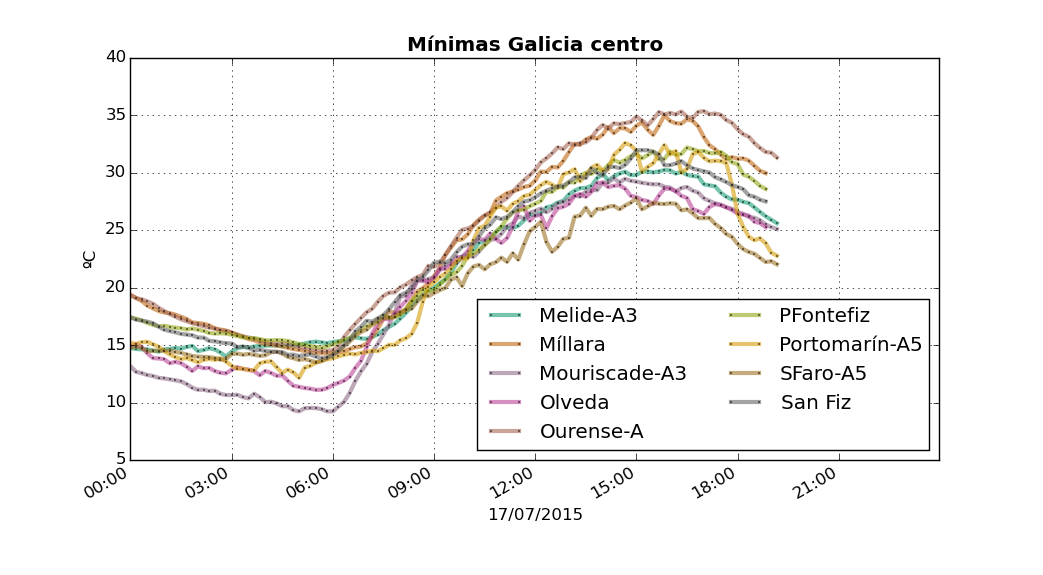
\includegraphics[width = 1.0 \textwidth]{images/presentacion/grafica.png}
\end{block}
\begin{block}{Animación da velocidade do vento}
\animategraphics[width = 1.0 \textwidth,loop,autoplay]{1}{images/presentacion/animacion/frame}{00}{30}
%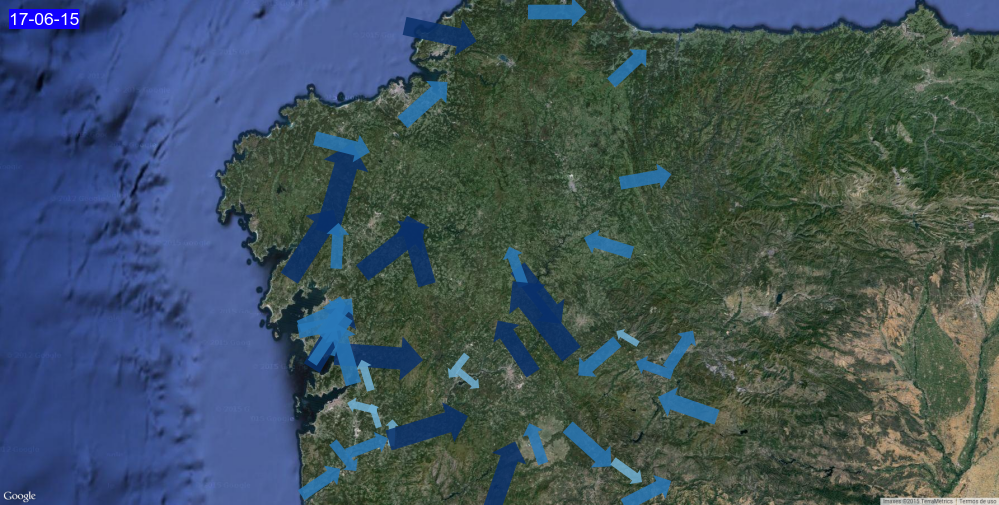
\includegraphics[width = 1.0 \textwidth]{images/presentacion/animacion/frame00.png}
\end{block}
\end{frame}

\section{Conclusións}
\begin{frame}{Conclusións e traballo futuro}
\onslide<1->{\begin{block}{Conclusións}
\begin{itemize}
\item Maior dificultade: Baixo nivel de implantación e madurez do estándar SOS.
\item Obxectivo cumprido: Soporte para os servidores SOSVDI do CiTIUS.
\item Aprobación do plugin no repositorio oficial de QGIS.
\end{itemize}
\end{block}}
\onslide<2->{\begin{block}{Traballo futuro}
\begin{itemize}
\item Sensor Observation Service 2.0.
\item Soporte de máis tipos de Observations\&Measurements.
\item Ampliación da funcionalidade de visualización de gráficas.
\item Funcionalidades para a visualización en tempo real.
\end{itemize}
\end{block}}
\end{frame}

\section*{}
\begin{frame}[plain]{\inserttitle}{\insertauthor}
	\transdissolve
	\begin{center}
		\textbf{\Huge {\usebeamercolor[bg]{title} Grazas pola súa atención!}}\\
		\bigskip
		\large{Dúbidas e comentarios?}
	\end{center}
\end{frame}

\end{document}